% (c) 2012 Tiziana Manca - tmanca@libero.it
% (c) 2012-2014 Dimitrios Vrettos - d.vrettos@gmail.com
%===================================
\section{Esercizi}
%===================================
\subsection{Esercizi dei singoli paragrafi}
%===================================
\subsubsection*{7.1 - Proposizioni e predicati}

\begin{esercizio}
\label{ese:7.1}
Completa la tabella come suggerito nella prima riga, individuando, per ciascuna proposizione, il predicato e gli argomenti a cui esso si riferisce:
\begin{center}
\begin{tabular}{llc}
\toprule
Proposizioni & Predicato & Argomenti\\
\midrule
7 è divisore di~14 & essere divisore di & 7, 14 \\
11 è maggiore di~10 & essere maggiore di & \\
5 è numero primo & & \\
Andrea frequenta la stessa palestra di Marco & & \\
Marta è moglie di Piero & & \\
Paolo è padre di Marco & & \\
\bottomrule
\end{tabular}
\end{center}
\end{esercizio}

%===================================
\subsubsection*{7.2 - Relazioni in un insieme}
\begin{esercizio}
\label{ese:7.2}
Nell'insieme~$A = \{$3, 5, 6, 9, 30$\}$ considera il predicato ``essere minore di''; con esso forma proposizioni vere aventi come soggetto e come complemento due elementi di~$A$.

\emph{Esempio}: $p_1$: 9\text{ è minore di }30.
\end{esercizio}

\begin{esercizio}
\label{ese:7.3}
Nell'insieme~$A$ rappresentato con il diagramma di Eulero-Venn di figura~\ref{fig:7.10} introduciamo il predicato~$\Rel$: ``avere
una sola lettera diversa''. Costruisci l'insieme~$G_\Rel$.

\begin{figure}[b]
\begin{minipage}[b]{.45\textwidth}
 \centering
 % (c) 2012 Dimitrios Vrettos - d.vrettos@gmail.com

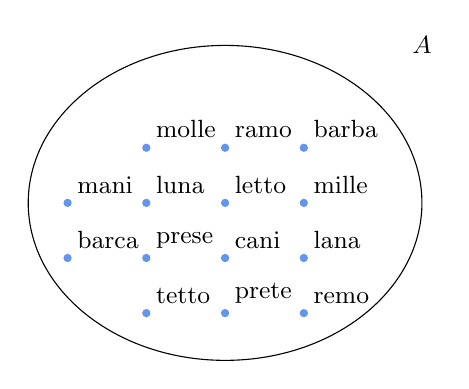
\begin{tikzpicture}[x=10mm,y=10mm, font=\small]
\draw (0,0) circle [x radius=2.5, y radius=2];

\node  at (2.5,2) {$A$};
 \begin{scope}[fill=CornflowerBlue]
\fill (0,0) circle (1.5pt) node[above right] {letto};
\fill (-1,0) circle (1.5pt) node[above right] {luna};
\fill (-2,0) circle (1.5pt) node[above right] {mani};
\fill (-2,-.7) circle (1.5pt) node[above right] {barca};
\fill (1,0) circle (1.5pt) node[above right] {mille};
\fill (0,.7) circle (1.5pt) node[above right] {ramo};
\fill (1,.7) circle (1.5pt) node[above right] {barba};
\fill (-1,.7) circle (1.5pt) node[above right] {molle};
\fill (0,-.7) circle (1.5pt) node[above right] {cani};
\fill (1,-.7) circle (1.5pt) node[above right] {lana};
\fill (-1,-.7) circle (1.5pt) node[above right] {prese}; 
\fill (0,-1.4) circle (1.5pt) node[above right] {prete};
\fill (1,-1.4) circle (1.5pt) node[above right] {remo};
\fill (-1,-1.4) circle (1.5pt) node[above right] {tetto}; 
 \end{scope}
\end{tikzpicture}
 \caption{}\label{fig:7.10}
\end{minipage}\hfil
\begin{minipage}[b]{.45\textwidth}
 \centering
 % (c) 2012 Dimitrios Vrettos - d.vrettos@gmail.com
\begin{tikzpicture}[scale=.5, x=7.5mm, y=7.5mm, font=\scriptsize]
\begin{scope}[->]
\draw (0,0) -- (0,7.5);
\draw (0,0) -- (7.5,0);
\end{scope}

\begin{scope}[Maroon, dotted, step=7.5mm]
\draw (0,0) grid (7.5,7.5);
\end{scope}

\foreach \x/\xtext in {1/lunedì,2/martedì}{
\node[below left=.2, rotate=30] at (\x,0) {\xtext};
\node[left=.15] at (0,\x) {\xtext};
}
\begin{scope}[very thick, draw=CornflowerBlue, decoration={crosses, shape size=1.5mm}]
\draw decorate {(1,1) -- (1,1.1)};
\draw decorate {(2,2) -- (2,2.1)};
\end{scope}
\end{tikzpicture}
 \caption{}\label{fig:7.11}
\end{minipage}
\end{figure}

\emph{Traccia di soluzione}:
Per costruire l'insieme~$G_\Rel$ devo formare le coppie ordinate ricordando che per qualunque~$a$ e~$b$ appartenenti ad~$A$, $a \,\Rel\, b$
se e solo se ``$a$ ha una sola lettera diversa da~$b$'', ad esempio prete$\,\Rel\,$prese.
\end{esercizio}

\begin{esercizio}
\label{ese:7.4}
Nell'insieme~$C = \{$Como, Milano, Venezia, Parma, Brescia, Aosta, Torino, Genova, Imperia, Arezzo,
Firenze, Grosseto, Napoli, Campobasso, Catanzaro, Bologna, Vercelli, Salerno$\}$ è definita la
relazione~$\Rel$: ``essere nella stessa regione''. Costruisci l'insieme~$G_\Rel$.
\end{esercizio}

\begin{esercizio}
\label{ese:7.5}
Nell'insieme~$S = \{ x \mid  x$ è il nome di un giorno della settimana$\}$ è definita la
relazione~$\Rel$:~$x \in S$, $y \in S$, $x \,\Rel\, y$ se e solo se ``$x$ ha
lo stesso numero di sillabe di~$y$''. Costruisci l'insieme~$G_\Rel$.
\end{esercizio}

\begin{esercizio}
\label{ese:7.6}
Nell'insieme~$F = \{$1, 3, 4, 6, 5, 9, 0, 2$\}$ è definita la relazione~$\Rel$: ``essere consecutivi''. Costruisci l'insieme~$G_\Rel$.
\end{esercizio}

 \begin{esercizio}
\label{ese:7.7}
Considera l'insieme~$S = \{ x \mid  x$ è il nome di un giorno della settimana$\}$, completa la rappresentazione grafica di figura~\ref{fig:7.11} a pagina~\pageref{fig:7.11}, dell'insieme~$S \times S$,
evidenzia poi con una crocetta gli elementi dell'insieme~$G_\Rel$ determinato dalla relazione ``$x$ ha lo stesso numero di sillabe di~$y$''.
\end{esercizio}

\begin{esercizio}
\label{ese:7.8}
Considera l'insieme~$F = \{$1, 3, 4, 6, 5, 9, 0, 2$\}$; fai la rappresentazione grafica dell'insieme~$F \times F$ e metti in evidenza con una crocetta gli
elementi dell'insieme~$G_\Rel$ determinato dalla relazione ``essere consecutivi''.
\end{esercizio}

\begin{esercizio}
\label{ese:7.9}
Considera nell'insieme~$A = \{-1$, $+3$, $-7$, $+5$, $-2$, $+4$, $+10\}$ la relazione~$\Rel$:~$x \in A$, $y \in A$, $x \Rel y$ se e solo se ``$x$
è concorde con~$y$''. Costruiamo una tabella a doppia entrata (figura~\ref{fig:7.12}) riportando in orizzontale e in verticale gli elementi dell'insieme~$A$.
Fissa l'attenzione su una cella e segui le istruzioni:
\begin{itemize*}
\item se~$a \,\Rel\, b$ metti~1 nella cella~$(a;b)$;
\item altrimenti metti~0 nella cella~$(a;b)$.
\end{itemize*}
Prosegui tu seguendo l'esempio.
\end{esercizio}

\osservazione Alla fine tutte le celle sono riempite: compare zero se gli elementi della coppia ordinata non sono in relazione, compare~1 al contrario.
La relazione~$\Rel$ è completamente rappresentata.

La tabella costruita si chiama \emph{matrice della relazione}.
Una relazione può sempre essere rappresentata attraverso una matrice.

\begin{esercizio}
\label{ese:7.10}
Nell'insieme~$S = \{ x \mid  x$ è il nome di un giorno della settimana$\}$ è introdotta la relazione~$\Rel$:~$x \in S$, $y \in S$, $x \,\Rel\, y$
se e solo se ``$x$ ha lo stesso numero di sillabe di~$y$''. Rappresenta la relazione con una matrice.
\end{esercizio}

\begin{esercizio}
\label{ese:7.11}
Assegnato il predicato~$\Rel$: ``essere divisibile per'' introdotto nell'insieme~$A =\{$12, 4, 2, 8, 3, 21, 5, 60$\}$, rappresenta con una matrice la relazione~$\Rel$.
\end{esercizio}

\begin{figure}[b]
\begin{minipage}[b]{.45\textwidth}
 \centering
 % (c) 2012 Dimitrios Vrettos - d.vrettos@gmail.com

\begin{tikzpicture}[x=10mm,y=10mm, font=\small,table nodes/.style={%
		rectangle,
		draw=black,
 		align=center,
   		minimum height=5mm,
     	text depth=0.5ex,
     	text height=1.5ex,
     	inner xsep=-1pt,
     	outer sep=0pt
	},
	table/.style={%
        matrix of nodes,
        row sep=-\pgflinewidth,
        column sep=-\pgflinewidth,
        nodes={%
            table nodes
        } }]

\matrix (first) [table,text width=7mm,name=table,row 2 column 2/.style=blue,row 5 column 4/.style=blue]
{
{}  & $-1$ & $+3$ & $-7$ & $+5$ & $-2$ & $+4$ & $+10$\\
$-1$ &[blue] 1 &{} &{} &{} &{} &{} &{} \\
$+3$ &{} &{} &{} &{} &{} &{} &{} \\
$-7$ &{} &{} &{} &{} &{} &{} &{} \\
$+5$ &{} &{} &{$0$} &{} &{} &{} &{} \\
$-2$ &{} &{} &{} &{} &{} &{} &{} \\
$+4$ &{} &{} &{} &{} &{} &{} &{} \\
$+10$ &{} &{} &{} &{} &{} &{} &{} \\
};

\end{tikzpicture}
 \caption{}\label{fig:7.12}
\end{minipage}\hfil
\begin{minipage}[b]{.45\textwidth}
 \centering
 % (c) 2012 Dimitrios Vrettos - d.vrettos@gmail.com

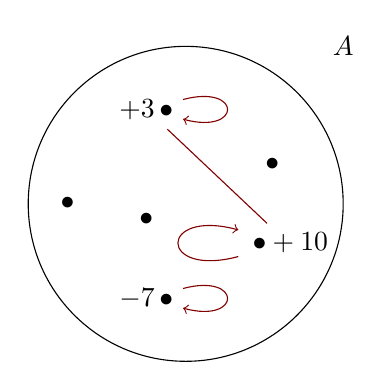
\begin{tikzpicture}[x=10mm,y=10mm, every state/.style={draw=CornflowerBlue}, every loop/.style={draw=Maroon}]
\draw (0,0) circle (2);
\node at (2,2) {$A$};
\node[]  at (-1.5,0) {$\bullet$};
\node[] (3) at (-.5,1.2) {$+3 \, \bullet$};
\node[]  at (1.1,.5) {$\bullet$};
\node[]  at (-.5,-.2) {$\bullet$};
\node[] (10) at (1.3,-.5) {$\, \bullet+10$};
\node[] (7) at (-.5,-1.2) {$-7\, \bullet $};

\begin{scope}[->]
\path (3) edge[loop right] node{} ()
	(10) edge[loop left] node{} ()
   (7) edge[loop right] node {} ();

\end{scope}
\begin{scope}[-, Maroon]
\draw[] (10)--(3);
\end{scope}
\end{tikzpicture}
 \caption{}\label{fig:7.13}
\end{minipage}
\end{figure}

\begin{esercizio}
\label{ese:7.12}
Completa la rappresentazione di figura~\ref{fig:7.13} a pagina~\pageref{fig:7.13} con le frecce relative alla relazione~$\Rel$:~$x \in A$, $y \in A$, $x \Rel y$ se e solo se ``$x$ è concorde con~$y$''
nell'insieme~$A =\{-1$, $+3$, $-7$, $+5$, $-2$, $+4$, $+10\}$.
\end{esercizio}

\begin{esercizio}
\label{ese:7.13}
Nell'insieme~$A = \{$1, 2, 3, 4, 5, 6, 7, 8, 9$\}$ è introdotto il predicato~$\Rel$: ``essere il
doppio di''; costruisci l'insieme~$G_\Rel$, rappresenta la relazione nei tre modi descritti sopra: con un grafico cartesiano,
con una matrice e con un grafo.
\end{esercizio}

\begin{esercizio}
\label{ese:7.14}
Sono assegnati i grafi di tre relazioni~$\Rel_1$, $\Rel_2$, $\Rel_3$ definite in altrettanti insiemi~$A$, $B$, $C$ (figura~\ref{fig:7.14}); deduci da essi gli elementi di ciascun
insieme e costruisci, per ciascuna relazione, l'insieme~$G_\Rel$.
\end{esercizio}

\begin{esercizio}
\label{ese:7.15}
Rappresenta nei tre modi che sono stati descritti (con un grafico cartesiano, con una matrice, con un
grafo) la relazione~$\Rel$: ``essere nati nello stesso mese'' introdotta nell'insieme~$C$ degli alunni della tua classe.
\end{esercizio}

\begin{esercizio}
\label{ese:7.16}
Nell'insieme~$H = \{ x \in \insN \mid  21 < x < 40 \}$, $x \,\Rel\, y$ se e solo se ``la somma delle cifre di~$x$ è uguale alla somma delle cifre di~$y$''.
Costruisci~$G_\Rel$ e rappresenta la relazione con una matrice.
\end{esercizio}

\begin{esercizio}
\label{ese:7.17}
Rappresenta con un grafo la relazione~$\Rel$ indicata dal grafico cartesiano riportato nella figura~\ref{fig:7.15}.
\end{esercizio}

\begin{figure}[b]
\begin{minipage}[b]{.69\textwidth}
 \centering
 % (c) 2012 Dimitrios Vrettos - d.vrettos@gmail.com

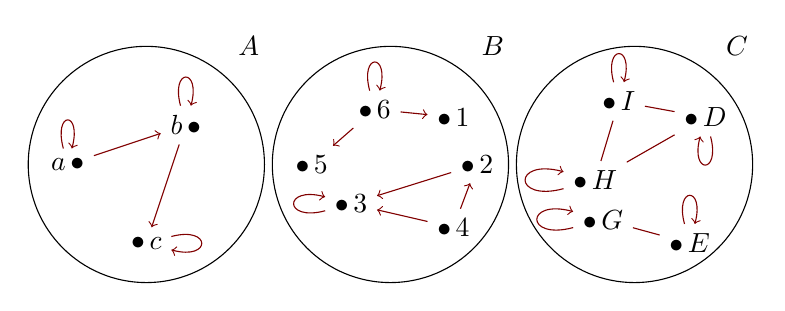
\begin{tikzpicture}[x=10mm,y=10mm, every state/.style={draw=CornflowerBlue, minimum size=0pt}, every loop/.style={draw=Maroon}]
\draw (0,0) circle (1.5);
\node at (1.3,1.5) {$A$};
\node[] (A) at (-1,0) {$a\, \bullet$};
\node[] (B) at (.5,.5) {$b\, \bullet$};
\node[] (C) at (0,-1) {$\bullet\, c$};

\begin{scope}[->]
\path (A) edge[loop above] node{} ()
	(B) edge[loop above] node{} ()
   (C) edge[loop right] node {} ();

\end{scope}
\begin{scope}[->, Maroon]
\draw (A)--(B);
\draw (B)--(C);
\end{scope}

\begin{scope}[xshift=31mm]
\draw (0,0) circle (1.5);
\node at (1.3,1.5) {$B$};
\node[] (1) at (.8,.6) {$\bullet\, 1$};
\node[] (2) at (1.1,0) {$\bullet\, 2$};
\node[] (3) at (-.5,-.5) {$\bullet\, 3$};
\node[] (4) at (.8,-.8) {$\bullet\, 4$};
\node[] (5) at (-1,0) {$\bullet\, 5$};
\node[] (6) at (-.2,.7) {$\bullet\, 6$};

\begin{scope}[->]
\path (6) edge[loop above] node{} ()
	(3) edge[loop left] node {} ();

\end{scope}
\begin{scope}[->, Maroon]
\draw (6)--(1);
\draw (6)--(5);
\draw (4)--(2);
\draw (4)--(3);
\draw (2)--(3);
\end{scope}
\end{scope}

\begin{scope}[xshift=62mm]
\draw (0,0) circle (1.5);
\node at (1.3,1.5) {$C$};
\node[] (D) at (.9,.6) {$\bullet\, D$};
\node[] (E) at (.7,-1) {$\bullet\, E$};
\node[] (G) at (-.4,-.7) {$\bullet\, G$};
\node[] (H) at (-.5,-.2) {$\bullet\, H$};
\node[] (I) at (-.2,.8) {$\bullet\, I$};

\begin{scope}[->]
\path (I) edge[loop above] node{} ()
	(H) edge[loop left] node {} ()
(G) edge[loop left] node {} ()
(E) edge[loop above] node {} ()
(D) edge[loop below] node {} ();

\end{scope}
\begin{scope}[-, Maroon]
\draw (D)--(I);
\draw (I)--(H);
\draw (D)--(H);
\draw (G)--(E);
\end{scope}
\end{scope}
\end{tikzpicture}
 \caption{}\label{fig:7.14}
\end{minipage}\
\begin{minipage}[b]{.3\textwidth}
 \centering
 % (c) 2012 Dimitrios Vrettos - d.vrettos@gmail.com
\begin{tikzpicture}[ x=7.5mm, y=7.5mm, font=\small]
\begin{scope}[->]
\draw (0,0) -- (0,3.5) node[left] {$y$};
\draw (0,0) -- (3.5,0) node[below] {$x$};
\end{scope}

\begin{scope}[Maroon, dotted, step=7.5mm]
\draw (0,0) grid (3.5,3.5);
\end{scope}

\foreach \x/\xtext in {1/1,2/2,3/3}{
\node[below] at (\x,0) {\xtext};
\node[left] at (0,\x) {\xtext};
}
\foreach \x in {1,2,3}{
\draw (\x,1.5pt) -- (\x,-1.5pt);
\draw (1.5pt,\x) -- (-1.5pt,\x);}
\node[below left] at (0,0) {0};
\begin{scope}[very thick, draw=CornflowerBlue, decoration={crosses, shape size=1.5mm}]
\draw decorate {(1,1) -- (1,1.1)};
\draw decorate {(2,2) -- (2,2.1)};
\draw decorate {(1,3) -- (1,3.1)};
\draw decorate {(2,1) -- (2,1.1)};
\draw decorate {(3,2) -- (3,2.1)};
\draw decorate {(3,3) -- (3,3.1)};
\end{scope}
\end{tikzpicture}
 \caption{}\label{fig:7.15}
\end{minipage}
\end{figure}
%\pagebreak

\subsubsection*{7.3 - Proprietà delle relazioni}

\begin{esercizio}
\label{ese:7.18}
Quali relazioni sono riflessive?
\begin{center}
\begin{tabular}{llc}
\toprule
Insieme & Relazione & È riflessiva?\\
\midrule
Numeri naturali & essere divisibile per & \boxSi\quad\boxNo \\
Libri che hai in cartella & avere lo stesso numero di pagine di & \boxSi\quad\boxNo \\
Rette del piano & essere perpendicolare a & \boxSi\quad\boxNo \\
Rette del piano & essere parallela a & \boxSi\quad\boxNo \\
Poligoni & avere lo stesso numero di lati di & \boxSi\quad\boxNo \\
Città della Lombardia & terminare con la stessa vocale & \boxSi\quad\boxNo \\
Parole italiane & essere il plurale di & \boxSi\quad\boxNo \\
\bottomrule
\end{tabular}
\end{center}
\end{esercizio}

%\subsubsection*{7.7 - Proprietà antiriflessiva}

\begin{esercizio}
\label{ese:7.19}
Quali delle seguenti relazioni sono antiriflessive?
\begin{center}
\begin{tabular}{llc}
\toprule
Insieme & Relazione & È antiriflessiva?\\
\midrule
Numeri naturali & essere multiplo di & \boxSi\quad\boxNo \\
Rette del piano & essere perpendicolare a & \boxSi\quad\boxNo \\
Poligoni & avere lo stesso perimetro & \boxSi\quad\boxNo \\
Città del Piemonte & avere più abitanti di & \boxSi\quad\boxNo \\
Parole italiane & essere il femminile di & \boxSi\quad\boxNo \\
Fiumi italiani & essere affluente di & \boxSi\quad\boxNo \\
Persone & essere figlio di & \boxSi\quad\boxNo \\
\bottomrule
\end{tabular}
\end{center}
\end{esercizio}

%\subsubsection*{7.8 - Proprietà simmetrica}

\begin{esercizio}
\label{ese:7.20}
Riconosci le relazioni simmetriche:
\begin{center}
\begin{tabular}{llc}
\toprule
Insieme & Relazione & È simmetrica?\\
\midrule
Città d'Italia & appartenere alla stessa regione & \boxSi\quad\boxNo \\
Rette del piano & essere perpendicolare a & \boxSi\quad\boxNo \\
Solidi & avere lo stesso volume di & \boxSi\quad\boxNo \\
Persone & essere il padre di & \boxSi\quad\boxNo \\
Persone & essere fratello o sorella di & \boxSi\quad\boxNo \\
Numeri naturali & avere lo stesso numero di cifre di & \boxSi\quad\boxNo \\
Fiumi d'Europa & essere affluente di & \boxSi\quad\boxNo \\
Numeri interi & essere il quadrato di & \boxSi\quad\boxNo \\
Persone & abitare nello stesso comune & \boxSi\quad\boxNo \\
\bottomrule
\end{tabular}
\end{center}

Le relazioni degli ultimi due casi non godono della proprietà simmetrica. Infatti:
\begin{itemize*}
\item la proposizione ``Il Ticino è un affluente del Po'' è vera, ma non lo è la proposizione che da essa si
ottiene scambiando il soggetto con il complemento;
\item se un numero intero è il quadrato di un altro (ad esempio~$+25$ è il quadrato di~$+5$), non è vero il contrario (infatti~$+5$ non è il quadrato di~$+25$).
\end{itemize*}
\end{esercizio}

\begin{esercizio}
\label{ese:7.21}
Riconosci le relazioni antisimmetriche:
\begin{center}
\begin{tabular}{llc}
\toprule
Insieme & Relazione & È antisimmetrica?\\
\midrule
Numeri naturali & essere divisibile per & \boxSi\quad\boxNo \\
Rette del piano & essere perpendicolare a & \boxSi\quad\boxNo \\
Poligoni & avere lo stesso perimetro di & \boxSi\quad\boxNo \\
Angoli & essere complementare a & \boxSi\quad\boxNo \\
Città del Lazio & essere nella stessa provincia di & \boxSi\quad\boxNo \\
\bottomrule
\end{tabular}
\end{center}
\end{esercizio}

\begin{esercizio}
\label{ese:7.22}
Verifica se, nell'insieme ~$\insN$ dei numeri naturali, la relazione~$\Rel$: ``avere lo stesso numero di cifre'' gode della proprietà transitiva.
Completa le proposizioni e rappresenta~$\Rel$ con un grafo:

\begin{enumeratea}
\item da~$18 \,\Rel\,50$ e~$50 \,\Rel\, \ldots$ segue~$\ldots \,\Rel\, \ldots$;
\item da~$\ldots \,\Rel\,555$ e~$\ldots \,\Rel\,267$ segue~$\ldots \,\Rel\, \ldots$
\end{enumeratea}
\end{esercizio}
\pagebreak
\begin{esercizio}
\label{ese:7.23}
Indica quale tra le seguenti relazioni è transitiva:
\begin{center}
\begin{tabular}{llc}
\toprule
Insieme & Relazione & È transitiva?\\
\midrule
Numeri naturali & essere multiplo di & \boxSi\quad\boxNo \\
Regioni d'Italia & essere più a nord di & \boxSi\quad\boxNo \\
Numeri interi & essere minore di & \boxSi\quad\boxNo \\
Rette del piano & essere perpendicolare a & \boxSi\quad\boxNo \\
Persone & essere padre di & \boxSi\quad\boxNo \\
Stati d'Europa & confinare con & \boxSi\quad\boxNo \\
\bottomrule
\end{tabular}
\end{center}
\end{esercizio}

\begin{esercizio}
\label{ese:7.24}
Dai una rappresentazione tabulare dell'insieme~$H = \{ x \in \insN \mid  0 \le x \le~12 \}$; determina il resto della divisione di ciascun numero di~$H$ con~4,
compila la tabella come suggerito nell'esempio:
\begin{center}
\begin{tabular}{lccccccccccccc}
\toprule
operazione & $0:4$ & $1:4$ & $2:4$ &\ldots & & & & & & & & $11:4$ & $12:4$ \\
resto & 0 & 1 &\ldots & & & & & & & & & 3 & 0 \\
\bottomrule
\end{tabular}
\end{center}
Introduciamo in~$H$ la relazione~$x \,\Rel\, y$ se e solo se ``$x$ e~$y$ hanno lo stesso resto nella divisione per~4''.
Costruisci il grafo della relazione e stabilisci se gode della proprietà transitiva.

La stessa relazione~$\Rel$, introdotta nell'insieme dei numeri naturali~$\insN$ è una relazione transitiva?
\end{esercizio}

\begin{esercizio}
\label{ese:7.25}
Indica le proprietà che verificano le seguenti relazioni.
\begin{center}
(R=riflessiva, S=simmetrica, T=transitiva, AS=antisimmetrica, AR=antiriflessiva)

\begin{tabular}{llc}
\toprule
Insieme & Relazione & Proprietà\\
\midrule
Poligoni del piano & avere lo stesso numero di lati & [R] \, [S]\, [T]\, [AS]\, [AR] \\
Numeri naturali & avere lo stesso numero di cifre & [R] \, [S]\, [T]\, [AS]\, [AR] \\
Numeri naturali & essere minore di & [R] \, [S]\, [T]\, [AS]\, [AR] \\
Numeri naturali & essere divisibile per & [R] \, [S]\, [T]\, [AS]\, [AR] \\
$A = \{ x \in \insN \mid  1 \le x \le~5 \}$ & essere multiplo di & [R] \, [S]\, [T]\, [AS]\, [AR] \\
Auto & essere della stessa marca costruttrice & [R] \, [S]\, [T]\, [AS]\, [AR] \\
\bottomrule
\end{tabular}
\end{center}
\end{esercizio}

%\pagebreak
\subsubsection*{7.4 - Relazioni di equivalenza}

\begin{esercizio}
\label{ese:7.26}
Quali delle seguenti sono relazioni di equivalenza?
\begin{center}
\begin{tabular}{llc}
\toprule
Relazione & Insieme & È d'equivalenza?\\
\midrule
Essere multiplo & numeri naturali & \boxV\quad\boxF \\
Avere lo stesso numero di sillabe & parole italiane & \boxV\quad\boxF\\
Essere minore & interi relativi & \boxV\quad\boxF \\
Vincere & squadre di calcio & \boxV\quad\boxF\\
Avere lo stesso numero di angoli & poligoni & \boxV\quad\boxF \\
Essere il plurale & parole italiane & \boxV\quad\boxF \\
Essere il cubo & numeri italiani & \boxV\quad\boxF \\
\bottomrule
\end{tabular}
\end{center}
\end{esercizio}

\begin{multicols}{2}
\begin{esercizio}
\label{ese:7.27}
Fissa l'attenzione sulla relazione~$\Rel$: ``frequentare la stessa classe'' introdotta nell'insieme~$S$ degli alunni iscritti nella tua scuola.
Verifica che~$\Rel$ è una relazione d'equivalenza. Costruisci le classi d'equivalenza. Quante ne hai potute formare? Come sono indicate nella
realtà che vivi quotidianamente? Determina la partizione~$P(S)$ in classi d'equivalenza e infine l'insieme quoziente~$S/\Rel$.
\end{esercizio}

\begin{esercizio}
\label{ese:7.28}
Studia in~$\insN$ la relazione~$\Rel$: ``avere la stessa cifra delle unità''. Verifica se è una relazione
d'equivalenza, costruisci l'insieme quoziente dopo aver risposto alle seguenti domande:\vspace{-1ex}
\begin{itemize*}
\item quanti numeri naturali sono tra loro equivalenti?
\item da quanti elementi è costituito l'insieme~$\insN/\Rel$?
\item qual è l'elemento che sceglieresti come rappresentante di ciascuna classe?
\end{itemize*}
\end{esercizio}

\begin{esercizio}
\label{ese:7.29}
Considera la relazione~$\Rel$: ``avere lo stesso resto nella divisione per due'' introdotta nell'insieme~$\insN$ e studiane le proprietà.
\begin{itemize*}
\item è una relazione d'equivalenza? Se la risposta è affermativa, costruisci l'insieme quoziente~$\insN/\Rel$.
\item quante classi d'equivalenza hai formato?
\item puoi sfruttare quanto ottenuto per enunciare le definizioni di numero pari e di numero dispari?
\item giustifica, in base allo svolgimento dell'esercizio, l'affermazione: ``L'insieme dei numeri pari è il
complementare in~$\insN$ dell'insieme dei numeri dispari''.
\end{itemize*}
\end{esercizio}

\begin{esercizio}
\label{ese:7.30}
Considera l'insieme~$A = \{x\in\insN \mid  1 \le x \le~20 \}$ e i suoi
sottoinsiemi:~$A_1 =\{$1, 5, 9, 13, 17$\}$, $A_2 =\{$2, 6, 10, 14, 18$\}$, $A_3 =\{$3, 7, 11, 15, 19$\}$, $A_4 =\{$4, 8, 12, 16, 20$\}$.
\begin{enumeratea}
\item Rappresenta gli insiemi con un diagramma di Eulero-Venn;
\item si può affermare che quei sottoinsiemi costituiscono una partizione dell'insieme~$A$?
\item è vero che a ciascuno dei suddetti sottoinsiemi appartengono i numeri di~$A$ aventi lo stesso resto nella divisione per~4?
\item quei sottoinsiemi sono dunque classi d'equivalenza? Qual è il predicato della relazione che le determina?
\end{enumeratea}
\end{esercizio}

\begin{esercizio}
\label{ese:7.31}
Nell'insieme ~$\insN$ dei numeri naturali stabilisci se è d'equivalenza la relazione~$\Rel$: ``$x \,\Rel\, y$ se e solo se~$x$ ha le stesse cifre di~$y$''.
\end{esercizio}

\begin{esercizio}
\label{ese:7.32}
Nell'insieme~$C$ degli alunni della tua classe, verifica se la relazione~$\Rel$: ``$x \,\Rel\, y$ se e solo se il cognome di~$x$ ha la stessa lettera iniziale del
cognome di~$y$'' è d'equivalenza; determina in caso affermativo la partizione dell'insieme~$C$ e l'insieme quoziente~$C/\Rel$.
\end{esercizio}

\begin{esercizio}
\label{ese:7.33}
Nell'insieme delle parole della lingua italiana verifica se la relazione ``$x \,\Rel\, y$ se e solo se~$x$ ha lo stesso numero di lettere di~$y$'' è
una relazione di equivalenza. In caso affermativo individua alcune classi di
equivalenza.
\end{esercizio}

\begin{esercizio}
\label{ese:7.34}
Nell'insieme dei nomi dei giorni della settimana considera la relazione ``$x \,\Rel\, y$ se e solo se~$x$ e~$y$ scritti in lettere, hanno almeno tre lettere in comune''.
Verifica se è una relazione di equivalenza e in caso affermativo individua le
classi di equivalenza.
\end{esercizio}

\begin{esercizio}
\label{ese:7.35}
Nell'insieme dei numeri naturali da~1 a~100, verifica se la relazione ``$x \,\Rel\, y$ se e solo se~$x$ e~$y$ hanno lo stesso numero di lettere''
è una relazione di equivalenza. Individua quante sono le classi di equivalenza.
Scrivi tutti gli elementi delle classi di equivalenza~$[1]$ e~$[10]$.
\end{esercizio}

\begin{esercizio}
\label{ese:7.36}
Nell'insieme dei numeri naturali da~1 a~100, verifica se la relazione ``$x \,\Rel\, y$ se e solo se~$x+y$ è
dispari'' è una relazione di equivalenza.
\end{esercizio}

\begin{esercizio}
\label{ese:7.37}
Nell'insieme dei nomi dei mesi dell'anno verifica se la relazione ``$x \,\Rel\, y$ se e solo se~$x$ e~$y$ hanno lo stesso numero di giorni''
è una relazione di equivalenza. Eventualmente individua le classi di equivalenza.
\end{esercizio}
%\end{multicols}

%\begin{multicols}{2}
\subsubsection*{7.5 - Relazioni di ordine}
\begin{esercizio}
\label{ese:7.38}
Nell'insieme~$M =\{$1, 8, 3, 4, 10, 2, 7, 0, 5, 9, 6$\}$ viene introdotta la relazione~$\Rel$ così definita: ``$x \,\Rel\, y$ se e solo se~$y-x$ appartiene a ~$\insN$''.
La relazione è riflessiva? La relazione è antisimmetrica? La relazione è transitiva? \`E vero che due elementi
distinti sono sempre confrontabili?
\end{esercizio}

\begin{esercizio}
\label{ese:7.39}
Verifica che la relazione~$\Rel$: ``essere divisore'' introdotta nell'insieme~$J =\{$3, 6, 10, 15, 21$\}$ è una relazione d'ordine parziale in senso largo.
\end{esercizio}

\begin{esercizio}
\label{ese:7.40}
Perché la relazione~$\Rel$ rappresentata dal grafico cartesiano riportato nella figura, %~\ref{fig:B.21}, 
pur essendo una relazione d'ordine non può essere
classificata in nessuna delle tipologie studiate? Dai una breve motivazione indicando quali proprietà non sono soddisfatte dalla relazione rappresentata.
\begin{center}
% (c) 2012 Dimitrios Vrettos - d.vrettos@gmail.com
\begin{tikzpicture}[ x=7.5mm, y=7.5mm, font=\small]
\begin{scope}[->]
\draw (0,0) -- (0,4.5) node[left] {$y$};
\draw (0,0) -- (4.5,0) node[below] {$x$};
\end{scope}

\begin{scope}[Maroon, dotted, step=7.5mm]
\draw (0,0) grid (4.5,4.5);
\end{scope}

\foreach \x/\xtext in {1/5,2/7,3/10,4/20}{
\node[below] at (\x,0) {\xtext};
\node[left] at (0,\x) {\xtext};
}
\foreach \x in {1,2,3,4}{
\draw (\x,1.5pt) -- (\x,-1.5pt);
\draw (1.5pt,\x) -- (-1.5pt,\x);}
\node[below left] at (0,0) {0};
\begin{scope}[very thick, draw=CornflowerBlue, decoration={crosses, shape size=1.5mm}]
\draw decorate {(1,1) -- (1,1.1)};
\draw decorate {(1,2) -- (1,2.1)};
\draw decorate {(1,3) -- (1,3.1)};
\draw decorate {(1,4) -- (1,4.1)};
\draw decorate {(2,3) -- (2,3.1)};
\draw decorate {(2,4) -- (2,4.1)};
\draw decorate {(4,3) -- (4,3.1)};
\draw decorate {(4,4) -- (4,4.1)};
\end{scope}
\end{tikzpicture}
\end{center}
\end{esercizio}

\begin{esercizio}
\label{ese:7.41}
Nell'insieme degli studenti della tua classe determina le proprietà della relazione~$\Rel$: ``$x \,\Rel\, y$ se e solo se l'altezza di~$x$ non supera l'altezza di~$y$''. \`E una relazione d'ordine? Di quale tipo?
\end{esercizio}

\begin{esercizio}
\label{ese:7.42}
Nell'insieme~$A = \{$12, 4, 2, 8, 3, 21, 5, 60$\}$ la relazione~$\Rel$: ``essere divisibile'' è una relazione d'ordine? Se lo è, di che tipo di relazione si tratta? Totale, parziale, in senso largo, in senso stretto?
\end{esercizio}

\begin{esercizio}
\label{ese:7.43}
Nell'insieme ~$\insN - \{ 0 \}$ la relazione ``essere divisibile'' è d'ordine totale in senso largo?
\end{esercizio}
%\end{multicols}

\subsubsection*{7.6 - Relazioni tra due insiemi diversi}
\begin{esercizio}
\label{ese:7.44}
Rappresenta con un grafico cartesiano la relazione~$\Rel$: "essere nato nell'anno" di dominio l'insieme~$A=$ \{Galileo, Napoleone, Einstein, Fermi, Obama\}
e codominio l'insieme~$B=$\{1901, 1564, 1961, 1879, 1769, 1920, 1768\}. Rappresenta per elencazione il sottoinsieme~$G_\Rel$ del prodotto cartesiano~$A \times B$.
Stabilisci infine gli elementi dell'immagine~$\IM$.
\end{esercizio}

\begin{esercizio}
\label{ese:7.45}
L'insieme~$S=$ \{casa, volume, strada, ufficio, clavicembalo, cantautore, assicurazione\} è il codominio della relazione~$\Rel$: "essere il numero di sillabe di" il cui dominio
è~$X=\{x \in\insN / 0<x<10\}$. Rappresenta con un grafico cartesiano la relazione assegnata, evidenzia come nel primo esempio di questo paragrafo l'insieme~$G_\Rel$,
scrivi per elencazione l'insieme~$\IM$.
\end{esercizio}

\begin{esercizio}
\label{ese:7.46}
Completa la rappresentazione con grafico sagittale della relazione "essere capitale di". La freccia che collega gli elementi del dominio con quelli del codominio rappresenta
il predicato~$\Rel$: "essere la capitale di".
\begin{center}
 % (c) 2012 Dimitrios Vrettos - d.vrettos@gmail.com
\begin{tikzpicture}[x=10mm, y=10mm, scale=.8]

\node[ellipse, minimum height=2.5cm,draw, minimum width=3.5cm] (D) at (0,0) {};

\node[above] (D1) at (D.north) {$\Dom$};

\begin{scope}[fill=CornflowerBlue]

\filldraw (.7,1) circle (2pt) node (a) {};
\node[left] at (.7,1) {Roma};
\filldraw (1,.2) circle (2pt) node (b) {};
\node[left] at (1,.2) {Parigi};

\filldraw (-1.3,-.5) circle (2pt) node (c) {};
\end{scope}

\begin{scope}[xshift=5cm]
\node[ellipse, minimum height=2.5cm,draw, minimum width=3.5cm] (C) at (0,0) {};

\node[above] (C1) at (C.north) {$\Cod$};

\begin{scope}[fill=LimeGreen]
\filldraw (-.1,1) circle (2pt) node (a1) {};
\filldraw (-.2,.2) circle (2pt)node (b1) {};
\filldraw (.2,-.8) circle (2pt) node (c1) {};

\node[right]  at (-.1,1) {Francia};
\node[right]  at (.2,-.8) {Italia};
\node[right] at (-.2,.2) {Grecia};

\end{scope}
\end{scope}
\begin{scope}[->,smooth,thick]
\draw[red] (c) .. controls +(-30:2cm) and +(-180:2cm) .. (b1);
\end{scope}
\end{tikzpicture}
\end{center}
\end{esercizio}
%\subsubsection*{C.3 - Caratteristiche di una relazione}

\begin{esercizio}
\label{ese:7.47}
È univoca la relazione~$\Rel$ definita tra l'insieme~$P=$ \{parola del proverbio "rosso di sera, bel tempo si spera"\} e l'insieme~$A=$\{lettere dell'alfabeto italiano\}
che associa ad ogni parola la sua iniziale? Ti sembra corretto affermare che dominio e insieme di definizione coincidono? Completa con il simbolo corretto
la relazione tra insieme immagine e codominio:~$\IM\ldots\Cod$. Fai il grafico sagittale della relazione.
\end{esercizio}
\end{multicols}

\begin{esercizio}
\label{ese:7.48}
$\Rel$ è la relazione tra l'insieme ~$\insN$ dei naturali e l'insieme degli interi relativi~$\insZ$ espressa dal predicato "essere il quadrato di". Ti sembra corretto affermare che
dominio e insieme di definizione coincidono? Perché~$\IM=\Cod$? La relazione è univoca?
\end{esercizio}
%\newpage
\begin{esercizio}
\label{ese:7.49}
Una relazione~$\Rel$ è assegnata con il suo grafico cartesiano.
\begin{center}
 % (c) 2012 Dimitrios Vrettos - d.vrettos@gmail.com
\begin{tikzpicture}[x=10mm, y=10mm,scale=.8]

\begin{scope}[->]
\draw (-.5,0) -- (12,0);
\draw (0,-.5) -- (0,7);
\end{scope}

\foreach \x in {1,2,...,11}
\draw (\x,1.5pt) -- (\x,-1.5pt);

\foreach \y in {1,2,...,6}
\draw (1.5pt,\y) -- (-1.5pt,\y);

\foreach \xi/\xtext in {1/A,2/B,3/C,4/D,5/E,6/F,7/G,8/H,9/I,10/L,11/M}
\node[below] at (\xi,0) {$\xtext$};

\foreach \yi/\ytext in {1/1,2/2,3/3,4/4,5/5,6/6}
\node[left] at (0,\yi){\ytext};

\draw[orange, dotted] (0,0) grid (11,6);

\begin{scope}[fill=CornflowerBlue]
\foreach \x in {1,6}
\filldraw (\x,1) circle (2pt);

\foreach \x in {2,5,8}
\filldraw (\x,2) circle (2pt);

\foreach \x in {4,10}
\filldraw (\x,4) circle (2pt);

\filldraw (3,5) circle (2pt);
\filldraw (11,6) circle (2pt);
\end{scope}
\end{tikzpicture}
\end{center}
Completa e rispondi alle domande:

\begin{enumeratea}
\item $\Dom=$\{\dotfill\};
\item $\Cod=$\{\dotfill\};
\item $\ID=$\{\dotfill\};
\item $\IM=$\{\dotfill\};
\item la relazione è biunivoca?
\item 2 è l'immagine di quali elementi dell'insieme di definizione?
\item quale elemento del codominio è l'immagine di~$M$?
\end{enumeratea}
\end{esercizio}

\begin{esercizio}
\label{ese:7.50}
I tre grafici sagittali rappresentano altrettante corrispondenze, $\Rel_1$, $\Rel_2$, $\Rel_3$.
Completa per ciascuna di esse la descrizione schematizzata nel riquadro sottostante:
\begin{center}
 % (c) 2012 Dimitrios Vrettos - d.vrettos@gmail.com
\begin{tikzpicture}[x=10mm, y=10mm]

\node[circle, minimum height=2cm,draw] (A) at (0,0) {};

\node[above] (A1) at (A.north) {$A$};

\begin{scope}[fill=CornflowerBlue]

\filldraw (.5,.5) circle (2pt) node (a) {};
\node[left] at (.5,.5) {1};
\filldraw (.8,.2) circle (2pt) node (b) {};
\node[left] at (.8,.2) {2};
\filldraw (-.4,-.5) circle (2pt) node (c) {};
\node[left] at (-.4,-.5)  {3};
\filldraw (-.5,0) circle (2pt);
\node[left] at (-.5,0)  {4};
\filldraw (-.3,.5) circle (2pt);
\node[left] at (-.3,.5)  {5};
\end{scope}

\begin{scope}[xshift=2.3cm]
\node[circle, minimum height=2cm,draw] (B) at (0,0) {};

\node[above] (B1) at (B.north) {$B$};

\begin{scope}[fill=LimeGreen]
\filldraw (-.1,.6) circle (2pt) node (a1) {};
\filldraw (-.2,.2) circle (2pt)node (b1) {};
\filldraw (.2,-.7) circle (2pt) node (c1) {};
\filldraw(.5,-.2) circle (2pt);

\node[right]  at (-.1,.6) {$a$};
\node[right] at (-.2,.2) {$b$};
\node[right]  at (.2,-.7) {$c$};
\node[right] at (.5,-.2) {$d$};
\end{scope}
\end{scope}

\begin{scope}[->,smooth,thick]
\draw[Maroon] (a) .. controls +(30:1cm) and +(150:.5cm) .. (a1);
\draw[Maroon] (b) .. controls +(30:.5cm) and +(180:0.5cm) .. (b1);
\draw[Maroon] (c) .. controls +(30:1cm) and +(-90:1cm) .. (b1);
\draw[Maroon] (c) .. controls +(30:1cm) and +(-180:2cm) .. (c1);
\end{scope}

\begin{scope}[yshift=-2.5cm]
\matrix (m) [matrix of nodes]
{$\Dom=$&\ldots\\
$\Cod=$&\ldots\\
$\ID=$&\ldots\\
$\IM=$&\ldots\\
Tipo$=$&\ldots\\};
\end{scope}


\begin{scope}[xshift=4.6cm]

\node[circle, minimum height=2cm,draw] (A) at (0,0) {};

\node[above] (A1) at (A.north) {$A$};

\begin{scope}[fill=CornflowerBlue]

\filldraw (0,.7) circle (2pt) node (a) {};
\node[left] at (0,.7) {$a$};
\filldraw (.7,0) circle (2pt) node (b) {};
\node[left] at (.7,0) {$b$};
\filldraw (-.4,-.5) circle (2pt) node (c) {};
\node[left] at (-.4,-.5)  {$c$};
\end{scope}

\begin{scope}[xshift=2.3cm]
\node[circle, minimum height=2cm,draw] (B) at (0,0) {};

\node[above] (B1) at (B.north) {$B$};

\begin{scope}[fill=LimeGreen]
\filldraw (-.1,.6) circle (2pt) node (a1) {};
\filldraw (-.2,.2) circle (2pt)node (b1) {};
\filldraw (.2,-.7) circle (2pt) node (c1) {};

\node[right]  at (-.1,.6) {$m$};
\node[right] at (-.2,.2) {$n$};
\node[right]  at (.2,-.7) {$p$};
\end{scope}
\end{scope}

\begin{scope}[->,smooth,thick]
\draw[Maroon] (a) .. controls +(30:1cm) and +(180:1cm) .. (b1);
\draw[Maroon] (b) .. controls +(30:1cm) and +(180:1cm) .. (c1);
\draw[Maroon] (c) .. controls +(30:.5cm) and +(-180:2cm) .. (a1);
\end{scope}

\begin{scope}[yshift=-2.5cm]
\matrix (m) [matrix of nodes]
{$\Dom=$&\ldots\\
$\Cod=$&\ldots\\
$\ID=$&\ldots\\
$\IM=$&\ldots\\
Tipo$=$&\ldots\\};
\end{scope}
\end{scope}

\begin{scope}[xshift=9.2cm]
\node[circle, minimum height=2.cm,draw] (A) at (0,0) {};

\node[above] (A1) at (A.north) {$A$};

\begin{scope}[fill=CornflowerBlue]

\filldraw (.3,.7) circle (2pt) node (a) {};
\node[left] at (.3,.7) {1};
\filldraw (.6,.2) circle (2pt) node (b) {};
\node[left] at (.6,.2) {2};
\filldraw (-.3,-.5) circle (2pt) node (c) {};
\node[left] at (-.3,-.5)  {3};
\filldraw (-.5,0) circle (2pt) node (d){};
\node[left] at (-.5,0)  {4};

\end{scope}

\begin{scope}[xshift=2.3cm]
\node[circle, minimum height=2cm,draw] (B) at (0,0) {};

\node[above] (B1) at (B.north) {$B$};

\begin{scope}[fill=LimeGreen]
\filldraw (-.1,.6) circle (2pt) node (a1) {};
\filldraw (-.2,.2) circle (2pt)node (b1) {};
\filldraw (.1,-.8) circle (2pt) node (c1) {};
\filldraw(.5,-.1) circle (2pt) node (d1) {};
\filldraw(-.7,-.4) circle (2pt) node (e1) {};

\node[right]  at (-.1,.6) {$a$};
\node[right] at (-.2,.2) {$b$};
\node[right]  at (.1,-.8) {$c$};
\node[right] at (.5,-.1) {$d$};
\node[right] at (-.7,-.4) {$e$};
\end{scope}
\end{scope}

\begin{scope}[->,smooth,thick]
\draw[Maroon] (a) .. controls +(30:.5cm) and +(90:.5cm) .. (e1);
\draw[Maroon] (b) .. controls +(30:.5cm) and +(90:.5cm) .. (e1);
\draw[Maroon] (c) .. controls +(30:.5cm) and +(-180:2cm) .. (b1);
\draw[Maroon] (d) .. controls +(-30:2cm) and +(-120:1cm) .. (d1);
\end{scope}

\begin{scope}[yshift=-2.5cm]
\matrix (m) [matrix of nodes]
{$\Dom=$&\ldots\\
$\Cod=$&\ldots\\
$\ID=$&\ldots\\
$\IM=$&\ldots\\
Tipo$=$&\ldots\\};
\end{scope}
\end{scope}
\end{tikzpicture}
\end{center}
\end{esercizio}

\subsection{Esercizi riepilogativi}

\begin{esercizio}
\label{ese:7.51}
L'insieme~$G_\Rel$ di una relazione introdotta nell'insieme~$A = \{a$, $b$, $c$, $d$, $e\}$ è~$G_\Rel = \{ (a;a)$, $(a;b)$, $(b;b)$, $(d;d)$, $(c;d)$, $(d;e)$, $(e;e)\}$.
Quale delle seguenti affermazioni è vera
\begin{enumeratea}
\item $\Rel$ è una relazione antiriflessiva;
\item $\Rel$ è una relazione solo antisimmetrica;
\item $\Rel$ è una relazione riflessiva;
\item $\Rel$ è una relazione transitiva e antisimmetrica;
\end{enumeratea}
\end{esercizio}

\begin{esercizio}
\label{ese:7.52}
La relazione~$\Rel$: ``essere vicini di banco'' inserita nell'insieme degli alunni della tua classe è una
relazione d'equivalenza? \`E una relazione d'ordine?
\end{esercizio}

\begin{esercizio}
\label{ese:7.53}
I tre sottoinsiemi~$A_1 = \{$36, 135, 432$\}$, $A_2 = \{65\}$ e $A_3 = \{$66, $3\,522$, 93, 435$\}$ dell'insieme~$A = \{$36, 65, 66, 93, 135, 432, 435, $3\,522\}$ costituiscono una partizione dell'insieme~$A$? Sapresti trovare una caratteristica per gli elementi di ciascun sottoinsieme? $A_1$, $A_2$, $A_3$ sono classi d'equivalenza?
\end{esercizio}

\begin{esercizio}
\label{ese:7.54}
La relazione~$\Rel$: ``$x \,\Rel\, y$ se e solo se~$x$ sta nella stessa nazione di~$y$'' nell'insieme~$K= \{$Parigi, Madrid, Milano, Siviglia, Bari, Granada, Venezia, Lione$\}$
è d'equivalenza? Costruisci~$A/\Rel$.
\end{esercizio}

\begin{esercizio}
\label{ese:7.55}
Verifica se la relazione~$\Rel$ assegnata con la matrice rappresentata
sotto è d'equivalenza. In caso positivo determina la partizione dell'insieme~$A =\{\square, \lozenge, \infty, \nabla\}$ e l'insieme
quoziente~$A/\Rel$.

\begin{center}
\begin{tabular}{ccccc}
\toprule
 & $\square$ & $\lozenge$ & $\infty$ & $\nabla$\\
\midrule
 $\square$ & 1 & 1 & 0 & 0 \\
 $\lozenge$ & 1 & 1 & 0 & 0 \\
 $\infty$ & 0 & 0 & 1 & 1\\
 $\nabla$ & 0 & 0 & 1 & 1\\
\bottomrule
\end{tabular}
\end{center}
\end{esercizio}

\begin{esercizio}
\label{ese:7.56}
Associa a ciascun grafo della figura %~\ref{fig:B.22} a pagina~\pageref{fig:B.22} 
la corretta relazione d'ordine:
\begin{enumeratea}
\item ordine totale in senso largo;
\item ordine totale in senso stretto;
\item ordine parziale in senso largo;
\item ordine parziale in senso stretto.
\end{enumeratea}
\begin{center}
 % (c) 2012 Dimitrios Vrettos - d.vrettos@gmail.com
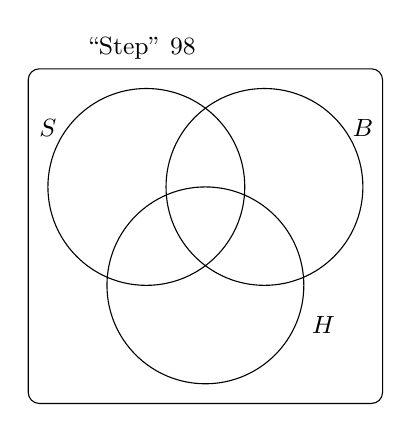
\begin{tikzpicture}[x=5mm, y=5mm,font=\small]

\draw[rounded corners] (0,-5.5) rectangle (9,3) (4.5,3)node[above, anchor=south east] {``Step'' 98};

\draw(3,0) circle (2.5);
\draw(6,0) circle (2.5);
\draw(4.5,-2.5) circle (2.5);

\node at (.5,1.5) {$S$};
\node at (8.5,1.5) {$B$};
\node at (7.5,-3.5) {$H$};

\end{tikzpicture}

\end{center}
\end{esercizio}
\pagebreak
\begin{esercizio}
\label{ese:7.57}
In un torneo di pallavolo gareggiano quattro squadre A, B, C, D; rappresenta con un grafo a frecce le seguenti informazioni, relative alle prime tre giornate:
\begin{itemize*}
\item 1\textsuperscript{a} giornata: A vince contro B; C vince contro D;
\item 2\textsuperscript{a} giornata: D vince contro A; B vince contro C;
\item 3\textsuperscript{a} giornata: A vince contro C; B vince contro D;
\end{itemize*}
Il~4\textsuperscript{o} giorno si gioca la semifinale tra le prime due classificate e le altre due. Se per ogni vittoria si ottiene un punteggio di~10 punti e per ogni sconfitta un punteggio
di~2 punti, quale squadra gioca la semifinale con B?
Il torneo è vinto dalla squadra C. Rappresenta con un grafo a frecce la situazione della semifinale e quella
della finale. \`E unica la risposta a quest'ultimo quesito?
\end{esercizio}

\begin{esercizio}
\label{ese:7.58}
Analizza le proprietà delle seguenti relazione e stabilisci se sono relazioni di equivalenza o di ordine e in questo caso di che tipo sono.
\begin{center}
\begin{tabular}{ll}
\toprule
Insieme & Relazione\\
\midrule
$\insN$ & $x \, \Rel \, y\, \Leftrightarrow\, x $ è la metà di~$ y $\\
$\insZ$ & $x \, \Rel \, y\, \Leftrightarrow\, x $ è il quadrato di~$ y $\\
$\insN$ & $x \, \Rel \, y\, \Leftrightarrow\, x+y\le x\cdot y $\\
Persone &$a \, \Rel \, b\, \Leftrightarrow\, a $ è più giovane di~$ b $ \\
Persone &$a \, \Rel \, b\, \Leftrightarrow\, a $ non è più vecchio di~$ b $ \\
Cittadini italiani &$a \, \Rel \, b\, \Leftrightarrow\, a $ risiede in una regione che confina con quella di~$ b $ \\
Rette del piano &$r \, \Rel \, s\, \Leftrightarrow\, r $ interseca $s$\\ 
Alunni della classe &$a \, \Rel \, b\, \Leftrightarrow\, a $ ha il nome con lo stesso numero di lettere di quello di~$ b $ \\
$\insZ$ & $a \, \Rel \, b\, \Leftrightarrow\, a^{2}=b^{2} $\\
Parole italiane & $p \, \Rel \, q\, \Leftrightarrow\, p=q $ oppure $ p $ precede $ q $ in uno specifico vocabolario\\
$\insN$ & $n \, \Rel \, m\, \Leftrightarrow\, n \cdot m $ è dispari\\
$\insN$ & $n \, \Rel \, m\, \Leftrightarrow\, n + m $ è dispari\\
Iscritti a Facebook &$a \, \Rel \, b\, \Leftrightarrow\, a $ ha più amici di~$ b $\\
Parole italiane & $p \, \Rel \, q\, \Leftrightarrow\, p $ ha meno lettere di~$ q $\\
$\insN$ & $n \, \Rel \, m\, \Leftrightarrow\, n $ ha lo stesso numero di cifre di~$ m $\\
Persone &$a \, \Rel \, b\, \Leftrightarrow\, a $ abita nella stessa via di~$ b $ \\
Persone &$a \, \Rel \, b\, \Leftrightarrow\, a $ parla la stessa lingua di~$ b $ \\
Persone &$a \, \Rel \, b\, \Leftrightarrow\, a $ ha lo stesso cognome di~$ b $ \\
$\insN$ & $n \, \Rel \, m\, \Leftrightarrow\, n $ ha un divisore diverso da~1 in comune con~$ m $\\
$\insZ$ & $x \, \Rel \, y\, \Leftrightarrow\, x\cdot y $ è negativo\\
\bottomrule
\end{tabular}
\end{center}
\end{esercizio}

\begin{esercizio}
\label{ese:7.59}
Andrea, insegnante di grafica, ha chiesto ai suoi alunni di usare il minimo numero di colori per colorare il modello della figura %~\ref{fig:B.23} a pagina~\pageref{fig:B.23},
sottostante in modo che poligoni confinanti non risultino con lo stesso colore. Come si può risolvere il problema? [Risposta: 3 colori]
\pagebreak

\emph{Traccia di soluzione}: Nell'insieme~$Z =\{$1, 2, 3, 4, 5, 6, 7, 8, 9$\}$ studia la relazione~$\Rel$: ``confinare con'', rappresentandola con un grafico cartesiano e sfrutta
i risultati trovati per risolvere il problema.
La soluzione può essere trovata fissando un punto interno a ciascuna regione: due punti sono uniti se e solo se le regioni confinano, il segmento che li congiunge
deve attraversare solo il loro confine comune; i punti che non sono congiunti indicano regioni che avranno lo stesso colore.
\begin{center}
 % (c) 2012 Dimitrios Vrettos - d.vrettos@gmail.com

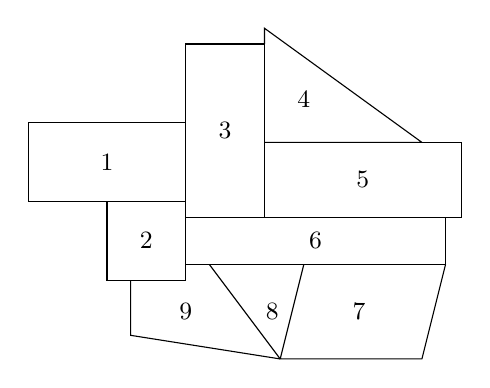
\begin{tikzpicture}[x=10mm,y=10mm, font=\small]
\draw (0,0) rectangle  (2,1) node[midway] {1};
\draw (1,-1) rectangle  (2,0) node[midway] {2};
\draw (2,-.2) rectangle  (3,2) node[midway] {3};
\draw (3,2)-- (3,2.2) -- (5,.75) --(3,.75);
\draw (3,.75) rectangle  (5.5,-.2) node[midway] {5};
\draw (2,-.2) rectangle  (5.3,-.8) node[midway] {6};
\draw (5.3,-.8) -- (5,-2) --(3.2,-2) --(3.5,-.8);
\draw (3.2,-2) -- (2.3,-.8);
\draw (3.2,-2) -- (1.3,-1.7)-- (1.3,-1);
 \node at (3.5,1.3) {4};
 \node at (4.2,-1.4) {7};
 \node at (3.1,-1.4) {8};
 \node at (2,-1.4) {9};
\end{tikzpicture}
\end{center}
\end{esercizio}
%\end{multicols}
%\pagebreak
